\chapter{Einleitung}

\section{Motivation}
\label{subsec:motivation}
Früher war alles besser. Nun ja, zumindest wenn es um das Auto geht trifft das nicht zu. Seit der Erfindung des ersten Motorwagens 1886, von Carl Benz, arbeiten Hersteller stetig weiter am Fahrzeug. Es wird immer komfortabler und vor allem sicherer. Dazu beigetragen haben zum Beispiel Erfindungen wie der Tempomat, der Airbag, das Antiblockiersystem oder das Navigationssystem, um nur einige der wichtigsten Erfindungen zu nennen.
Wer heutzutage keinen Einparkassistenten hat, der wird zumindest von Rückfahrkameras, Sensoren und akustischen Signalen unterstützt. 
Errungenschaften in der Automobilindustrie haben für weniger Unfälle mit schweren Personenschäden gesorgt. Heute gibt es bereits integrierte Notrufsysteme, wie den sogenannten eCall, der ab 2018 verpflichtend in allen Neuwagen eingebaut ist und noch mehr Sicherheit auf deutsche Straßen bringen soll. Kommt es zu einem Unfall wird automatisch Hilfe gerufen.
Wohin die Fahrt geht lässt sich nicht sicher prophezeien, aber eins steht fest: Ähnlich wie über die Diskette heute, wird in 20 Jahren über die automatische Einparkhilfe laut gelacht werden.\\  \\
\label{sec:einleitung}
\begin{figure}[htb]
  \centering  
  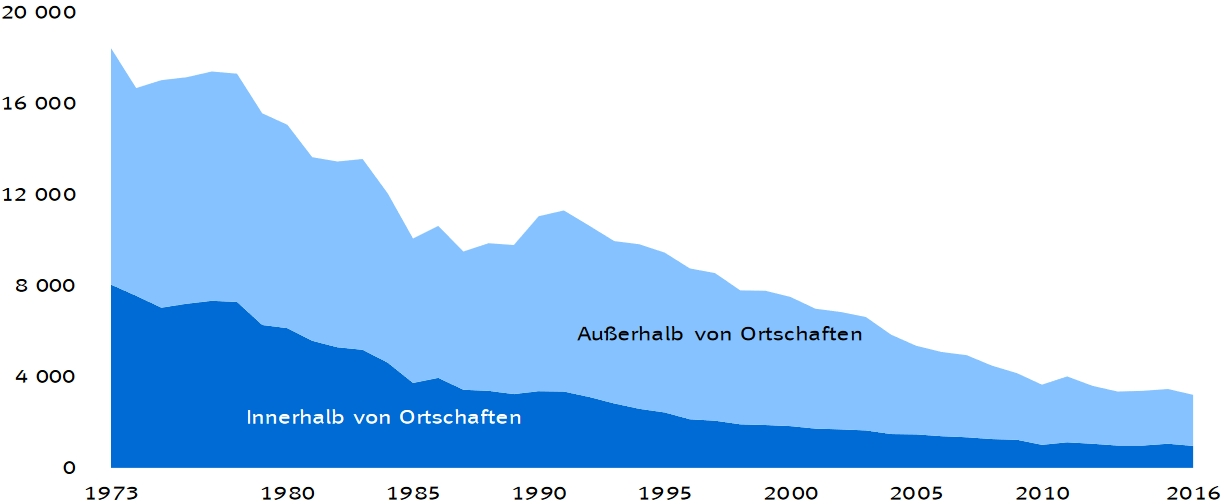
\includegraphics[scale=1.5]{img/Unfalle.jpg}
  \caption{Getötete nach Ortslagen 1973 - 2016\cite{bild1}}
  \label{fig:toteSeit1973}
\end{figure}
Trotz gestiegenem Verkehrsaufkommen sind sowohl die Zahl der Verletzten als auch der getöteten Menschen im Straßenverkehr bis heute stark gesunken. Abb. 1.1 zeigt die Entwicklung der Zahl der Unfallopfer in Deutschland seit dem Jahr 1973. Ein Grund für diesen fallenden Trend sind die eben genannten (und weitere) Fortschritte der Sicherheitssysteme durch die Automobilhersteller. Heute werden die meisten Unfälle durch Fehlverhalten der Fahrer verursacht, wie Abbildung 1.2 verdeutlicht. \\
\begin{figure}[htb]
  \centering  
  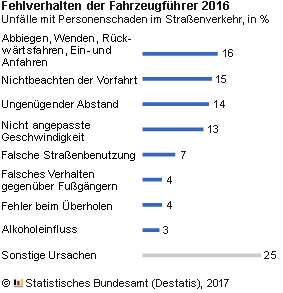
\includegraphics[scale=0.8]{img/Verkehrsunfaelle_Fehlverhalten.jpg}
  \caption{Fehlverhalten der Fahrzeugführer\cite{link}}
  \label{fig:Fehlverhalten}
\end{figure}
Laut Statistischem Bundesamt war im Jahr 2015 menschliches Fehlverhalten des Fahrers zu 88\% aller Unfälle mit Personenschaden die Ursache\cite{bild1}. \\
Dabei liegt in der fortschreitenden Automatisierung die Möglichkeit, Verkehrsunfälle bis auf ein Minimum zu reduzieren. \\
In dieser Bachelor Arbeit wird das Problem behandelt, ein System zu entwickeln, das sich anhand vorgegebener Koordinaten den optimalen Weg zum Ziel sucht und diesen dann möglichst genau abfährt. Die Problematik lässt sich also in zwei Unterprobleme aufteilen, dem Orientieren an einem passenden Pfad, sowie das Abfahren dieses. \\
Autonomes Fahren ist momentan ein Feld in dem viel geforscht wird. Die Automobilhersteller aller Länder liefern sich ein Wettrennen, doch so wie man das aus Science-Fiction Romanen kennt, funktionieren die Autos von heute noch nicht. Diese Arbeit dient der Grundlagenforschung auf diesem Gebiet. \newpage


\section{Problematik}
\label{subsec:problematik}
Um die Bewegung eines dynamischen Systems beschreiben zu können, müssen sich die auf das Fahrzeug wirkenden Kräfte genau angeschaut werden. Aus ihnen lassen sich Kräftegleichgewichte herleiten, mit deren Hilfe man zu den mathematischen Verhaltensbeschreibungen kommt, die möglichst genau die Realität abbilden sollen. 
Dabei lässt sich die Dynamik des Fahrzeugs in zwei Bereiche aufteilen, die Quer- und die Längsdynamik.
Die Freiheitsgrade Nicken und Hieven werden nicht behandelt. Bei der Betrachtung der Querdynamik werden die Bewegungen durch die Reibungskräfte zwischen
Straße und Reifen, sowie Kräfte und Momente der Aerodynamik beeinflusst.
Als Basis für die Regelung- und Steuereinheiten zur Bestimmung der Fahrzeugbewegung gilt
die Sollgrößendefinition, die das Regelziel festlegt. Die Fahrereingaben für das System sind Lenkradwinkel (querdynamisch) und Fahr- beziehungsweise Bremspedalstellung (längsdynamisch). Sie bilden die Basis der Interpretation des Fahrerwunsches, wenn auch nur imaginär, da weder bei der Simulation, noch beim Entwurf Lenker und Pedal tatsächlich enthalten sind. Das gesamte System wird anschließend mittels MATLAB/Simulink simuliert und auf einem RC-Auto mit Raspberry Pi realisiert. 
Diese Arbeit soll einen umfassenden Überblick über bereits veröffentlichte Fahrdynamikkennwerte verschiedener objektiver Fahrmanöver geben. 


\section{Überblick}
\label{subsec:überblick}
\begin{minipage}{0.4\textwidth}
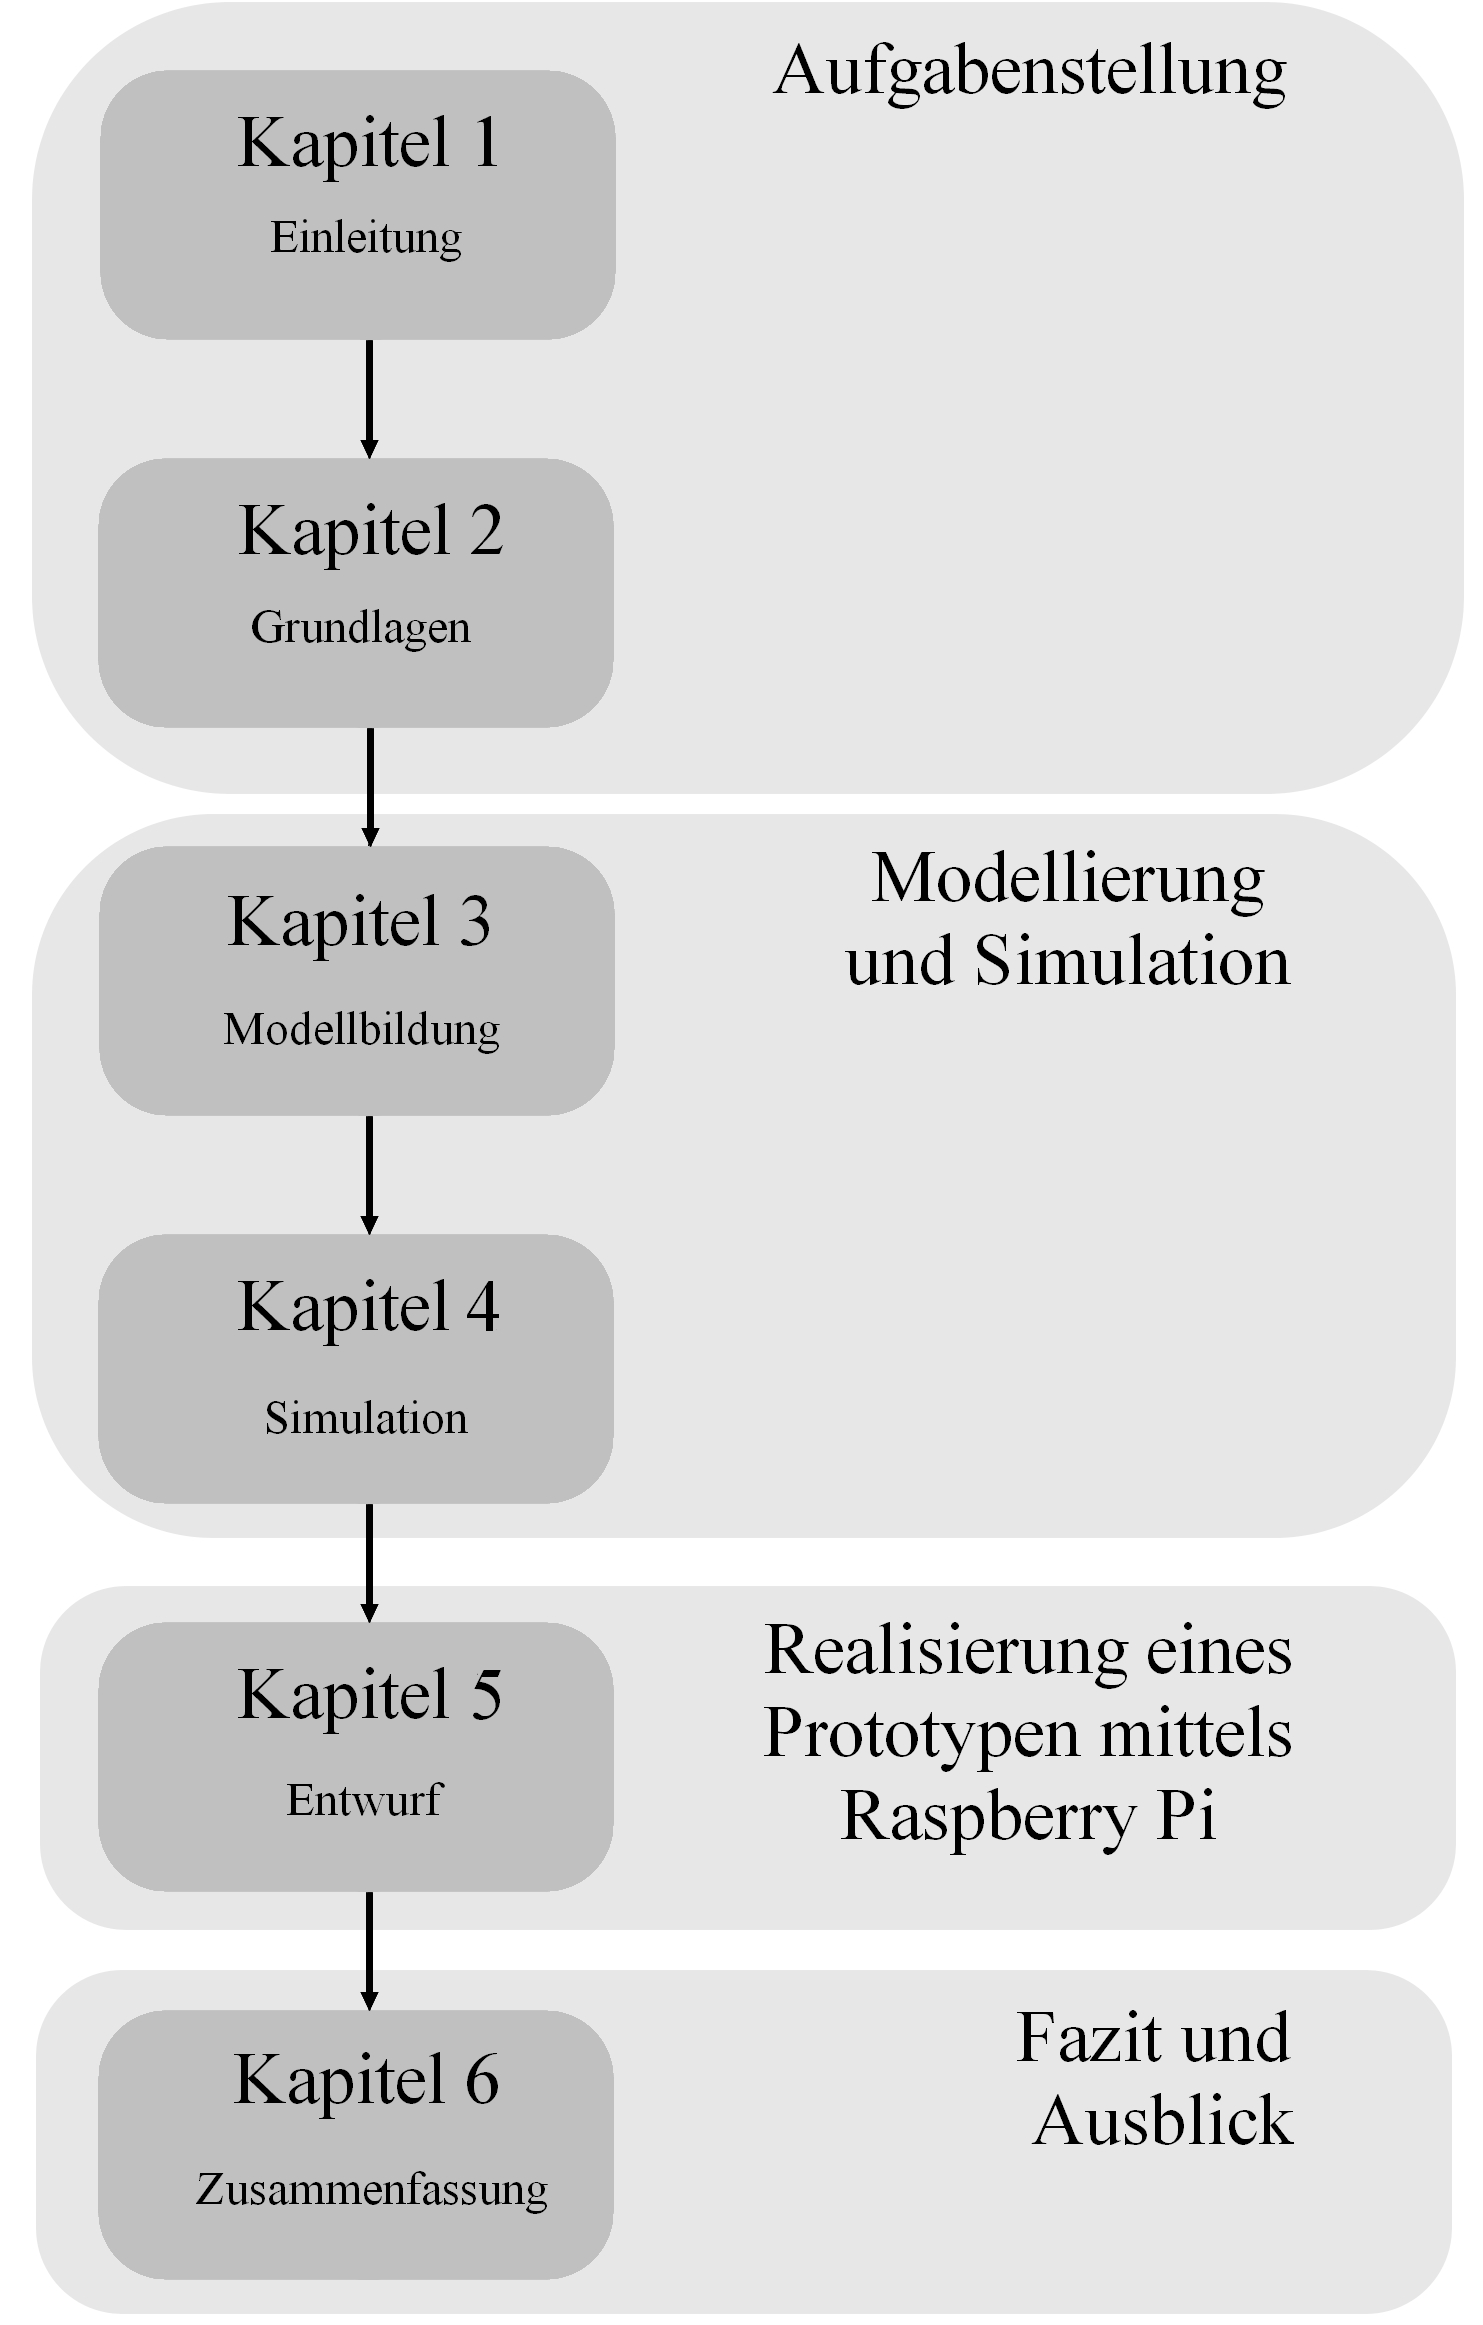
\includegraphics[width=\textwidth]{img/kapitel.jpg}
\end{minipage}
\begin{minipage}{0.6\textwidth}
Die vorliegende Arbeit ist in sechs Kapitel eingeteilt.
Die Kapitel bauen aufeinander auf und sind den einzelnen Teilproblemen der Aufgabenstellung gewidmet. \\
In Kapitel 2 geht es um die mathematischen und physikalischen Grundlagen, die zum Verständnis der folgenden Kapitel notwendig sind.
Kapitel 3 widmet sich der Modellbildung, sprich dem Erstellen mathematischer Formeln, die das Verhalten des Fahrzeugs aus der Aufgabenstellung möglichst realistisch wiedergeben. Es gibt bereits viele bewährte Ansätze und in diesem Fall wird bei dem Fahrzeug von einem Differentialmodell ausgegangen, d.h. einem Fahrzeug mit zwei Rädern und einem Stützrad. Zusätzlich wird hier die Aufgabe der Trajektorienfolgeregelung gelöst, also dem zeitlichen Sollverlauf des Abfahrens verschiedener Wegpunkte auf einem Koordinatensystem. \vspace{.15cm}
\end{minipage}
In Kapitel 4, der Simulation, wird gezeigt wie sich mit Hilfe von MATLAB/Simulink aus dem Modell ein Blockschaltbild erstellen lässt. Das Programm ermöglicht es dann, anhand dieses Blockschaltbilds das Verhalten zu simulieren. Ergebnisse der Simulationen können in dieser Arbeit nur als Bild gezeigt werden, wobei es eigentlich den Fahrvorgang in echtzeit visuell darstellt. In Kapitel 5 wird eine Architektur
entwickelt und die Realisierung eines Prototypen anhand eines Raspberry Pi beschrieben. Fokus hierbei ist die korrekte Ansteuerung der Pins, die wiederum die Aktuatoren des Fahrzeugs steuern sollen.
Im letzten Kapitel wird ein Fazit gezogen und erzielte Ergebnisse kritisch besprochen. Dann schließt diese Bachelorarbeit mit dem Ausblick.


\section{Stand der Technik}
Bislang kennen die meisten das autonome Fahren nur aus Science-Fiction-Büchern oder Filmen, dabei schleichen sich immer mehr autonome Funktionen zum Auto hinzu. So kann der Neuwagen von heute bereits den Abstand zum vorausfahrendem Fahrzeug messen, selbstständig einparken, die Spur halten und noch vieles mehr.
Die Society of Automotive Engineers (SAE) hat das autonome Fahren in sechs international allgemeingültige Stufen eingeteilt, von Level null "Keine Automation" bis zu Level fünf "vollautomatisiert" (vgl. Abbildung 1.3).

Beim Level null ist der Fahrer permanent für sein Fahrzeug verantwortlich, das manuell von ihm gesteuert wird. In Level eins wird der Fahrer von Fahrassistenzsystemen unterstützt, dieses greift aber nicht in Längs- oder Querführung ein. Der Stauassistent ist ein Beispiel für Level zwei, bei dem der Fahrer jedoch noch immer für alles verantwortlich ist (muss bereit sein einzuspringen), obwohl die Fahrzeugführung assistiert ist. Erst ab Level 3 ist es dem Fahrer erlaubt, die Verantwortung zeitweise an das Fahrzeug zu übertragen, muss allerdings aufmerksam bleiben, um für den Fall aller Fälle übernehmen zu können. Bei Level vier sind die ersten Funktionen komplett ohne Fahrer, das jedoch nur in bestimmten Situationen. Z.B. beim Parken oder auf der Autobahn. Das Auto kann in Level fünf in allen Verkehrssituationen auf allen Strecken ohne den Fahrer auskommen. Das Lenkrad ist bei Level fünf obsolet. Aktuell schaffen es die modernsten Autos lediglich auf Stufe 4. \\

Nach einem tödlichen Unfall in Arizona, in dem ein autonom fahrendes Fahrzeug verwickelt war, erlitten die Entwickler von selbst fahrenden Autos einen Rückschlag. Bei dem tragischen Unfall war eine Fußgängerin von einem selbst fahrenden Uber-SUV erfasst und getötet worden. \\
Dieser Vorfall zeigt, dass die Entwicklung am autonomen Fahren noch nicht abgeschlossen ist und unbedingt weitergehen muss. 
\begin{figure}[htb]
  \centering  
  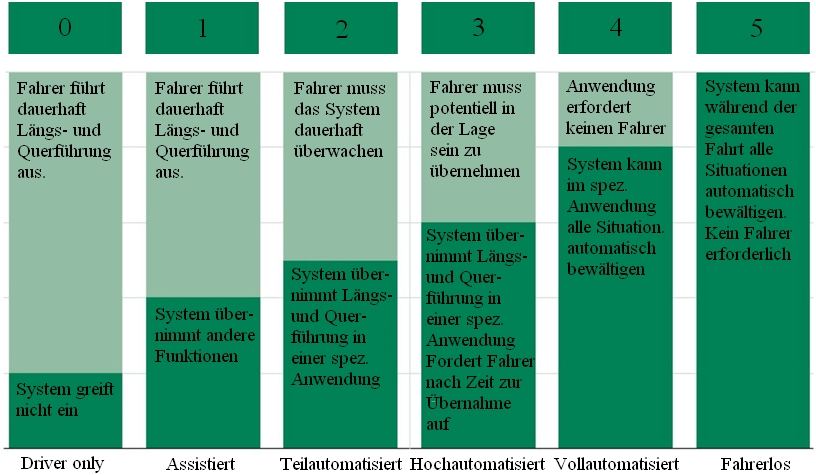
\includegraphics[scale=0.4]{img/automatisierungsgrad.jpeg}
  \caption{die fünf Stufen der Automatisierung}
  \label{fig:die fünf Stufen der Automatisierung}
\end{figure}



